\documentclass[border=1pt]{standalone}
\usepackage{mathptmx}
\usepackage[T1]{fontenc}
\usepackage{tikz}
\usetikzlibrary{positioning, arrows.meta, calc, fit, backgrounds, shapes.geometric}

% ---------------------------------------------------------------------------
% Okabe-Ito colour-blind-safe palette, one colour per role, used nowhere else.
% ---------------------------------------------------------------------------
\definecolor{okblue}{HTML}{56B4E9}       % data / images in flight
\definecolor{okgreen}{HTML}{009E73}      % trainable, gradients flow
\definecolor{okgrey}{HTML}{4D4D4D}       % frozen, no gradients
\definecolor{okorange}{HTML}{E69F00}     % derived / intermediate artefact
\definecolor{okpurple}{HTML}{CC79A7}     % language: generator + summary
\definecolor{okvermillion}{HTML}{D55E00} % supervision / loss / gate / stop-grad
\definecolor{bandbg}{HTML}{F7F7F7}

\begin{document}
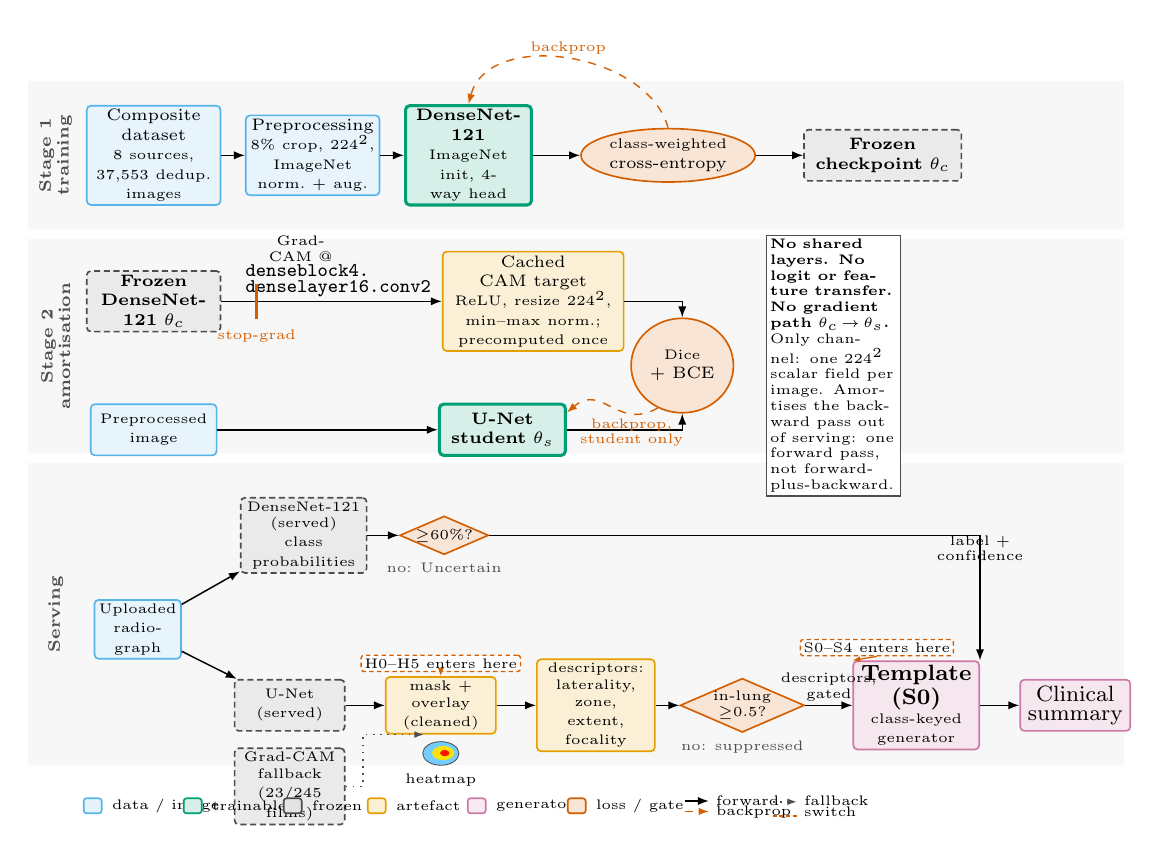
\begin{tikzpicture}[
    x=1in, y=1in,
    font=\fontsize{6.3}{7}\selectfont,
    >={Latex[length=1.4mm,width=1.05mm]},
    every node/.style={inner sep=1.4pt, font=\fontsize{6.3}{7}\selectfont},
    data/.style     ={rounded corners=1.5pt, draw=okblue,   fill=okblue!14,   line width=0.6pt},
    train/.style    ={rounded corners=1.5pt, draw=okgreen,  fill=okgreen!16,  line width=1.1pt},
    frozen/.style   ={rounded corners=1.5pt, draw=okgrey,   fill=okgrey!12,   line width=0.6pt, dash pattern=on 2.2pt off 1.3pt},
    artefact/.style ={rounded corners=1.5pt, draw=okorange, fill=okorange!16, line width=0.6pt},
    lang/.style     ={rounded corners=1.5pt, draw=okpurple, fill=okpurple!18, line width=0.6pt},
    proc/.style     ={align=center, minimum height=6.5mm},
    loss/.style     ={ellipse, draw=okvermillion, fill=okvermillion!16, line width=0.6pt, align=center, inner sep=1pt},
    gate/.style     ={diamond, draw=okvermillion, fill=okvermillion!16, line width=0.6pt, align=center, inner sep=0pt, aspect=2.3, font=\fontsize{5.4}{5.8}\selectfont},
    tag/.style      ={rounded corners=1pt, draw=okvermillion, fill=white, dash pattern=on 1.6pt off 1.2pt, line width=0.5pt, align=center, font=\fontsize{5}{5.4}\selectfont, inner sep=1.2pt},
    fwd/.style      ={-{Latex[length=1.4mm,width=1.05mm]}, solid, line width=0.55pt},
    sup/.style      ={-{Latex[length=1.3mm,width=0.95mm]}, dashed, line width=0.5pt, okvermillion},
    fallback/.style ={-{Latex[length=1.2mm,width=0.85mm]}, dotted, line width=0.6pt, okgrey},
    lbl/.style      ={font=\fontsize{5.1}{5.6}\selectfont, align=center},
    note/.style     ={draw=okgrey, line width=0.4pt, fill=white, align=left, font=\fontsize{5}{5.7}\selectfont},
  ]

% =====================================================================
% Band backgrounds. Bands stack bottom-up: legend, band 3, band 2, band 1.
% =====================================================================
\def\xR{5.15}
\begin{scope}[on background layer]
  \fill[bandbg] (-0.33,2.98) rectangle (\xR,3.72); % band 1
  \fill[bandbg] (-0.33,1.86) rectangle (\xR,2.93); % band 2
  \fill[bandbg] (-0.33,0.30) rectangle (\xR,1.81); % band 3
\end{scope}
\node[rotate=90, font=\fontsize{6}{6.4}\selectfont\bfseries, okgrey, align=center] at (-0.19,3.35) {Stage 1\\training};
\node[rotate=90, font=\fontsize{6}{6.4}\selectfont\bfseries, okgrey, align=center] at (-0.19,2.395) {Stage 2\\amortisation};
\node[rotate=90, font=\fontsize{6}{6.4}\selectfont\bfseries, okgrey, align=center] at (-0.19,1.055) {Serving};

% =====================================================================
% BAND 1: Stage 1, classifier training
% =====================================================================
\node[data, proc, text width=16mm] (s1-data) at (0.30,3.35) {Composite dataset\\{\tiny 8 sources, 37{,}553 dedup.\ images}};
\node[data, proc, text width=16mm, right=3mm of s1-data] (s1-pre) {Preprocessing\\{\tiny 8\% crop, $224^2$, ImageNet norm.\ + aug.}};
\node[train, proc, text width=15mm, right=3mm of s1-pre] (s1-net) {\textbf{DenseNet-121}\\{\tiny ImageNet init, 4-way head}};
\node[loss, minimum width=14mm, minimum height=6.5mm, right=6mm of s1-net] (s1-loss) {\tiny class-weighted\\cross-entropy};
\node[frozen, proc, text width=19mm, right=6mm of s1-loss] (s1-ckpt) {\textbf{Frozen}\\\textbf{checkpoint} $\theta_c$};

\draw[fwd] (s1-data) -- (s1-pre);
\draw[fwd] (s1-pre) -- (s1-net);
\draw[fwd] (s1-net) -- (s1-loss);
\draw[sup] (s1-loss.north) to[out=105,in=75] node[lbl,above,pos=0.5]{backprop} (s1-net.north);
\draw[fwd] (s1-loss) -- (s1-ckpt);

% =====================================================================
% BAND 2: Stage 2, explanation amortisation (never "distillation").
% Four visually distinct things: frozen teacher, stop-gradient, cached
% target, trainable student.
% =====================================================================
\node[frozen, proc, text width=16mm] (s2-teach) at (0.30,2.62) {\textbf{Frozen}\\\textbf{DenseNet-121} $\theta_c$};
\node[artefact, proc, text width=22mm, right=28mm of s2-teach] (s2-cam) {Cached CAM target\\{\tiny ReLU, resize $224^2$, min--max norm.; precomputed once}};
\node[data, proc, text width=15mm, below=9mm of s2-teach] (s2-img) {\tiny Preprocessed image};
\node[train, proc, text width=15mm, right=28mm of s2-img] (s2-unet) {\textbf{U-Net}\\\textbf{student} $\theta_s$};
\node[loss, minimum width=13mm, minimum height=12mm] (s2-loss) at ($(s2-cam.east)!0.5!(s2-unet.east)+(11mm,0)$) {\tiny Dice\\+ BCE};

\draw[fwd] (s2-teach.east) -- node[lbl, above, text width=14mm, pos=0.36]{Grad-CAM @\\\texttt{\scriptsize denseblock4.}\\\texttt{\scriptsize denselayer16.conv2}} (s2-cam.west);
\draw[okvermillion, line width=1.1pt] ($(s2-teach.east)+(4.5mm,-2.2mm)$) -- ++(0,4.4mm);
\node[okvermillion, font=\fontsize{4.6}{5}\selectfont, align=center] at ($(s2-teach.east)+(4.5mm,-4.4mm)$) {stop-grad};
\draw[fwd] (s2-img) -- (s2-unet);
\draw[fwd] (s2-cam.east) -| (s2-loss.north);
\draw[fwd] (s2-unet.east) -| (s2-loss.south);
\draw[sup] (s2-loss.240) to[out=210,in=40, looseness=1.3] node[lbl, below, pos=0.25, text width=15mm]{backprop,\\student only} (s2-unet.15);

\node[note, text width=16mm, right=4mm of s2-loss]
      (s2-note) {\textbf{No shared layers. No logit or feature transfer. No gradient path $\theta_c\!\to\!\theta_s$.} Only channel: one $224^2$ scalar field per image. Amortises the backward pass out of serving: one forward pass, not forward-plus-backward.};

% =====================================================================
% BAND 3: Serving, CPU, one request
% =====================================================================
\node[data, proc, text width=10mm] (s3-img) at (0.22,0.98) {\tiny Uploaded radiograph};

\node[frozen, proc, text width=15mm] (s3-cls) at (1.05,1.45) {\tiny DenseNet-121\\(served)\\class probabilities};
\node[gate, minimum width=7mm, right=4mm of s3-cls] (s3-gate1) {$\ge$60\%?};
\node[lbl, okgrey, below=0.4mm of s3-gate1] {no: Uncertain};

\node[frozen, proc, text width=13mm] (s3-loc) at (0.98,0.60) {\tiny U-Net (served)};
\node[frozen, proc, text width=13mm, minimum height=4.5mm, below=2mm of s3-loc] (s3-fb) {{\tiny Grad-CAM fallback\\(23/245 films)}};
\node[artefact, proc, text width=13mm, right=5mm of s3-loc] (s3-mask) {\tiny mask + overlay\\(cleaned)};
\node[artefact, proc, text width=14mm, right=5mm of s3-mask] (s3-desc) {\tiny descriptors:\\laterality, zone,\\extent, focality};
\node[gate, minimum width=9mm, right=3mm of s3-desc] (s3-gate2) {in-lung\\$\ge$0.5?};
\node[lbl, okgrey, below=0.4mm of s3-gate2] {no: suppressed};

\node[tag, above=0.5mm of s3-mask] (tagH) {H0--H5 enters here};
\draw[okvermillion, line width=0.45pt, -{Latex[length=1mm]}] (tagH.south) -- (s3-mask.north);

% small vector heatmap glyph under the mask node -- concentric blue/yellow/red
% "jet"-style ellipses, drawn, not a photo, illustrating what the overlay looks like
\begin{scope}[shift={($(s3-mask.south)+(0,-2.4mm)$)}]
  \fill[blue!35!cyan!55] (0,0) ellipse (2.3mm and 1.5mm);
  \fill[yellow!85!orange] (0.3mm,0.05mm) ellipse (1.4mm and 0.9mm);
  \fill[red!85!orange] (0.5mm,0.05mm) ellipse (0.6mm and 0.4mm);
  \draw[okgrey, line width=0.3pt] (0,0) ellipse (2.3mm and 1.5mm);
  \node[font=\fontsize{4.2}{4.6}\selectfont, below=0.5mm] at (0,-1.5mm) {\tiny heatmap};
\end{scope}

\node[lang, proc, text width=15mm, right=6mm of s3-gate2] (s3-rep) {\textbf{\footnotesize Template (S0)}\\{\tiny class-keyed generator}};
\node[tag, above=0.5mm of s3-rep, xshift=-5mm] (tagS) {S0--S4 enters here};
\draw[okvermillion, line width=0.45pt, -{Latex[length=1mm]}] (tagS.south) -- (s3-rep.north west);
\node[lang, proc, text width=13mm, right=5mm of s3-rep] (s3-sum) {\footnotesize Clinical\\summary};

\draw[fwd] (s3-img) -- (s3-cls);
\draw[fwd] (s3-img) -- (s3-loc);
\draw[fwd] (s3-cls) -- (s3-gate1);
\draw[fwd] (s3-loc) -- (s3-mask);
\draw[fallback] (s3-fb.east) -| ($(s3-fb.east)+(2.2mm,0)$) |- (s3-mask.240);
\draw[fwd] (s3-mask) -- (s3-desc);
\draw[fwd] (s3-desc) -- (s3-gate2);
\draw[fwd] (s3-gate1.east) -| node[lbl, pos=0.62, above, text width=16mm]{label + confidence} (s3-rep.north east);
\draw[fwd] (s3-gate2) -- node[lbl, pos=0.5, above, text width=13mm]{descriptors, gated} (s3-rep.west);
\draw[fwd] (s3-rep) -- (s3-sum);

% =====================================================================
% LEGEND
% =====================================================================
\begin{scope}[shift={(-0.05,0.06)}]
  \foreach \x/\col/\lbltxt [count=\i] in {
      0.00/okblue/{data / image},
      0.50/okgreen/{trainable},
      1.00/okgrey/{frozen},
      1.42/okorange/{artefact},
      1.92/okpurple/{generator},
      2.42/okvermillion/{loss / gate}} {
    \fill[\col!16, draw=\col, line width=0.6pt, rounded corners=1pt] (\x,0) rectangle ++(0.09,0.075);
    \node[font=\fontsize{4.7}{5}\selectfont, anchor=west] at (\x+0.12,0.0375) {\lbltxt};
  }
  \node[font=\fontsize{4.7}{5}\selectfont, anchor=west] at (2.98,0.065) {\tikz{\draw[fwd] (0,0) -- (0.12,0);} forward};
  \node[font=\fontsize{4.7}{5}\selectfont, anchor=west] at (2.98,0.008) {\tikz{\draw[sup] (0,0) -- (0.12,0);} backprop};
  \node[font=\fontsize{4.7}{5}\selectfont, anchor=west] at (3.42,0.065) {\tikz{\draw[fallback] (0,0) -- (0.12,0);} fallback};
  \node[font=\fontsize{4.7}{5}\selectfont, anchor=west] at (3.42,0.008) {\tikz{\draw[okvermillion, dash pattern=on 1.4pt off 1pt, line width=0.5pt] (0,0) -- (0.12,0);} switch};
\end{scope}

\end{tikzpicture}
\end{document}
